% !TEX program = xelatex

\documentclass{VUMIFPSkursinis}
\usepackage{algorithmicx}
\usepackage{algorithm}
\usepackage{algpseudocode}
\usepackage{amsfonts}
\usepackage{amsmath}
\usepackage{bm}
\usepackage{caption}
\usepackage{color}
\usepackage{float}
\usepackage{graphicx}
\usepackage{listings}
\usepackage{float}
\usepackage{subfig}
\usepackage{wrapfig}
\usepackage[hidelinks]{hyperref}
\usepackage{todonotes}
\usepackage{lineno}

% Titulinio aprašas
\university{Vilniaus universitetas}
\faculty{Matematikos ir informatikos fakultetas}
\department{}
\papertype{Programų sistemų inžinerijos modeliai ir metodai laboratorinis darbas 2}
\title{Requirements modeling}
\titleineng{Reikalavimų modeliavimas}
\status{1 course students}
\author{Matas Savickis}
\secondauthor{Vytautas Krivickas}
\thirdauthor{Šarūnas Kazimieras Buteikis}


\supervisor{Audronė Lupeikienė, M. Darbuot., Dr}
\date{Vilnius – \the\year}

% Nustatymai
% \setmainfont{Palemonas}   % Pakeisti teksto šriftą į Palemonas (turi būti įdiegtas sistemoje)
\bibliography{bibliografija}

\begin{document}
\selectlanguage{english}
\maketitle

\tableofcontents

\section{NFR type catalogue}

\begin{figure}[htbp]
	\center
	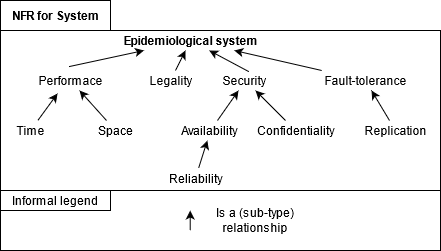
\includegraphics[scale=0.6]{img/1}
	\caption{NFR diagram} % Antraštė įterpiama po paveikslėlio
	\label{img:kurimoProcesas}
\end{figure}

	\begin{itemize}
		%\item{\textbf{Virus registration time} - to ensure quick response time system must provide quick process of registering new cases. }
		%\item{\textbf{Patient notification time} - it is important to prevent spread of virus by hastily notifying and isolating contagious patients.}
		%\item{\textbf{Holding medical records} - to ensure that the spread of the epidemic is contained and monitored, all necessary medical records related to the epidemic must be accessed via the system. }
		%\item{\textbf{Holding foreign countries data} - to check which countries are infected and are spreading the virus, the epidemiological system has to keep up-to-date epidemiological information about them.}
		\item{\textbf{Time} - System is monitoring the epidemic therefore it's processes or workflows have to be efficient time-wise.}
		\item{\textbf{Space} - since the system will contain lots of different data (e.g. person's geographical coordinates), data must be stored efficiently.}		
		\item{\textbf{Reliability} - Tracking the state of the epidemic must be ensured 24/7 to not miss any crucial data or trends.}
		\item{\textbf{Confidentiality} - epidemiological system must treat sensitive person information (e.g. received medical records) with respect to ensure systems credibility.}
		\item {\textbf{Legality} - due to the fact the the epidemiological system will deal with sensitive information, data handling must be in compliance with LT and EU data laws as well as GDPR.}
		\item{\textbf{Replication} - non sensitive data must have duplicate records stored to increase the system's fault-tolerance.}
	\end{itemize}

\section{Modelling of the non-functional requirements}
	\subsection{Time}
	\subsection{Space}
	\subsection{Legality}
	\subsection{Reliability}
	\subsection{Confidentiality}
	\subsection{Replication}

\section{Identifying and modelling of possible operationalizations for NFR}

\section{Detecting and modelling of implicit interdependencies among NFR}

\section{Chosen operationalizations}

\section{Strategic rationale model}

\section{Conclusions about an actor dependency}

\sectionnonum{Conclusions}

\end{document}
